\chapter{Results and Discussion}\label{ch:results-and-discussion}

\mycomment{
  * Chapter introduction
  * Results section
    > simulate a manual transcriber correcting results by ordering utterances using some metric and using specific WER caclulation
    > Run as average for single conversations AND whole corpus
    > present results using word-confidence
    > could make a table to show percentage of data checked versus reduction in WER?
  * Discussion section
    > average_logprob and utterance confidence are similar- appear to function well for average convo but poorly for whole corpus
    > explain: utterance confidence is calculated from the same logit data as utterance confidence (thus have similar shape)
    > explain word-confidence
    > works much better - long utterances can have few low-confidence words but get high average, word-confidence ordering eliminates this
    > word-confidence seems to work! there is benefit from using this metric
    > other two not so much
    > is this test representative of a real user?
    > by showing that there is a confidence metric which seems to work, Whisper is demonstrated to be a viable choice for aiding a human transcriber
    > perhaps work through requirements?
  * Future work (maybe a better title?)
    > try different type of confidence scoring - perhaps Whisper isn't the best candidate due to the way it makes choices?
    > try different datasets - LifeLUCID is only one out of thousand of corpora, try to replicate results
    > make fully-working transcription software - my example only shows the effect of ordering results, doesn't allow input
    > compare the effect of different model sizes - errors may be clustered differently - if smaller models could reliably get confidence then the hardware and time required to generate transcripts would be minimised
}

\section{Simulating Computer-Aided Transcription}

An effective computer-aided transcription system must reduce the human cost required to lower the amount of errors a transcription to an acceptable level.
By ordering transcribed utterances using some confidence metric and letting a human transcriber make corrections, an effective system should see the error rate fall more rapidly than if the results were corrected in a random order. \\

A simple simulation was devised in order to test the effectiveness of each potential measure of system confidence by using the formula for WER as follows;

\begin{enumerate}
  \item For a set of $M$ utterances $U = \{ u_{0}, u_{1}, \ldots\, u_{M} \}$ (either a single conversation or entire corpus), the subsitutions ($S_i$), deletions ($D_i$), insertions ($I_i$), and number of words in the reference ($N_i$) are calculated for each utterance, $u_i$.
  \item $U$ is ordered using a confidence metric.
  \item The WER, $w_i$, is calculated for a slice of $U$ containing all items including and following some utterance, $u_i$;
    \[
      w_i = \frac{\sum_{j=i}^{M} (S_j + D_j + I_j)}{\sum_{k=0}^{M} N_k}
    \]
  \item Increment $i$ by $1$ then repeat the previous step for all $0 \leq i \leq M$.
    Notice that the denominator is the same for all slices but the numerator changes to simulate each utterance being corrected in order.
  \item Output is a set $W = \{ w_{0}, w_{1}, \ldots\, w_{M} \}$, where some item $w_{i}$ is equal to the WER of $U$ after correcting all utterances prior to $u_i$.
\end{enumerate}

These results shall be analysed by plotting graphs of WER against the percentage of utterance which have been human-corrected, henceforth refered to as 'Cost'.

\section{Simulation Results}

This section details the results acquired from running this simple simulation using results ordered with each of the following metrics;

\begin{itemize}
  \item \texttt{avg\_logprob} taken directly from Whisper's standard output;
  \item utterance-average confidence score; and
  \item utterance minimum and maximum word-confidence scores.
\end{itemize}

\begin{figure}[p]
 \caption{Per-conversation average WER when evaluating in non-descending order of utterance \texttt{avg\_logprob}}
 \label{fig:average-avg-logprob}
 \centering
 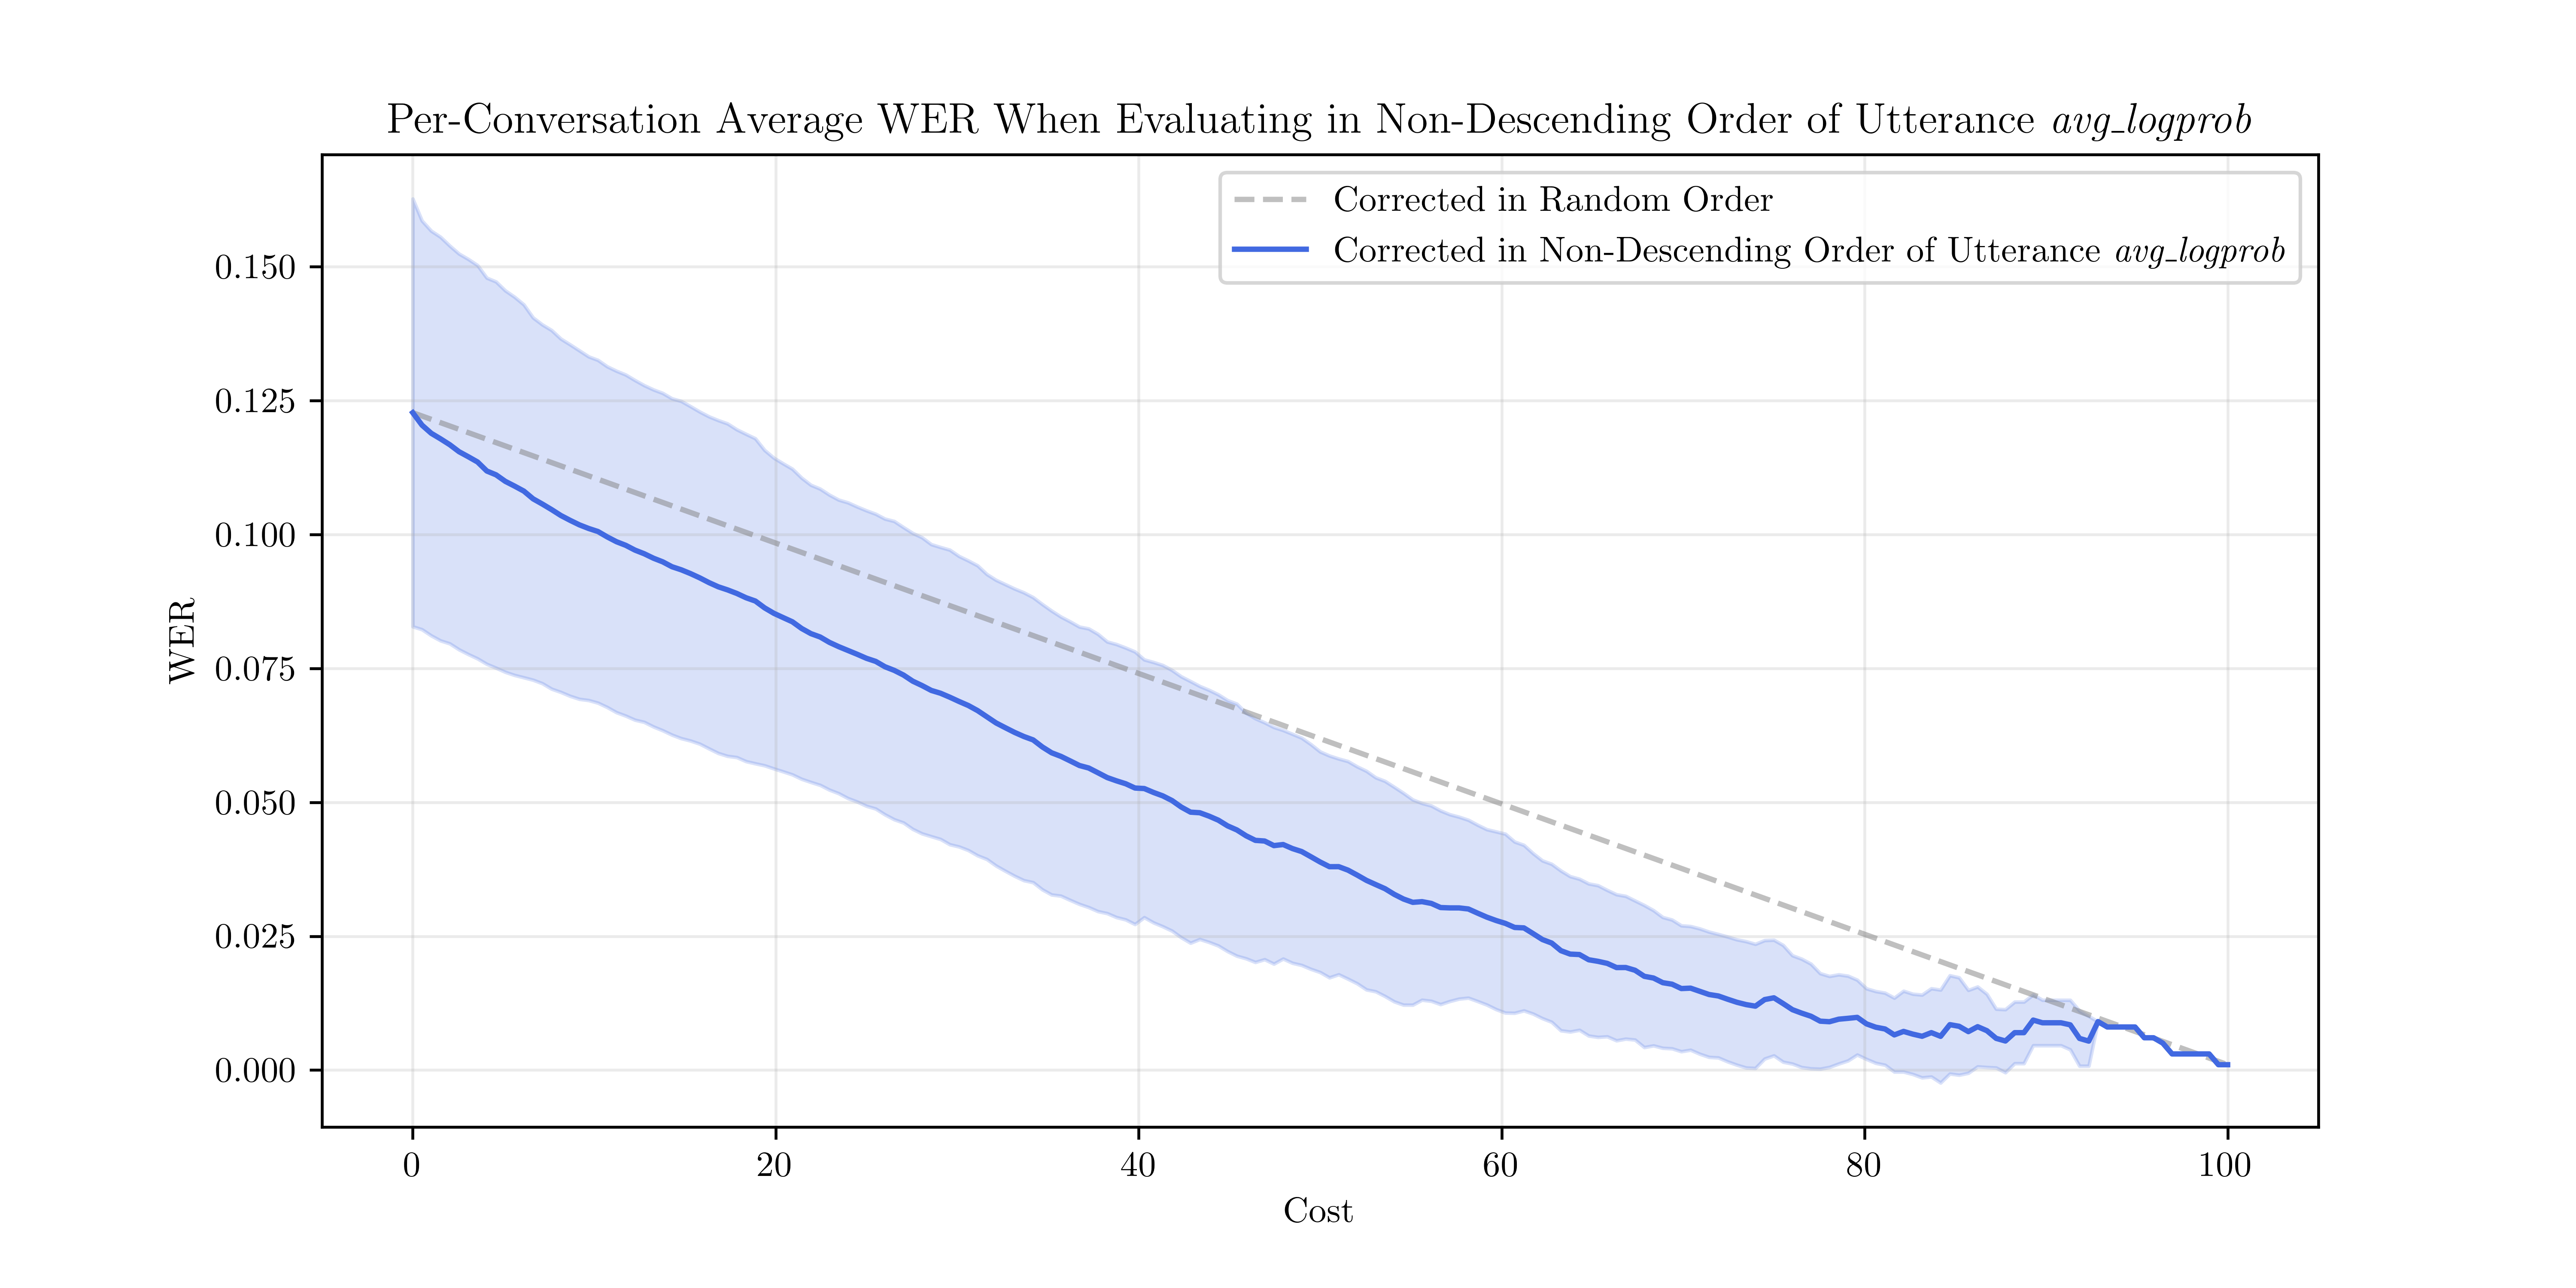
\includegraphics[width=\textwidth]{figures/average-avg-logprob.png}
\end{figure}
\begin{figure}[p]
 \caption{Per-conversation average WER when evaluating in non-descending order of utterance-average confidence}
 \label{fig:average-uttconf}
 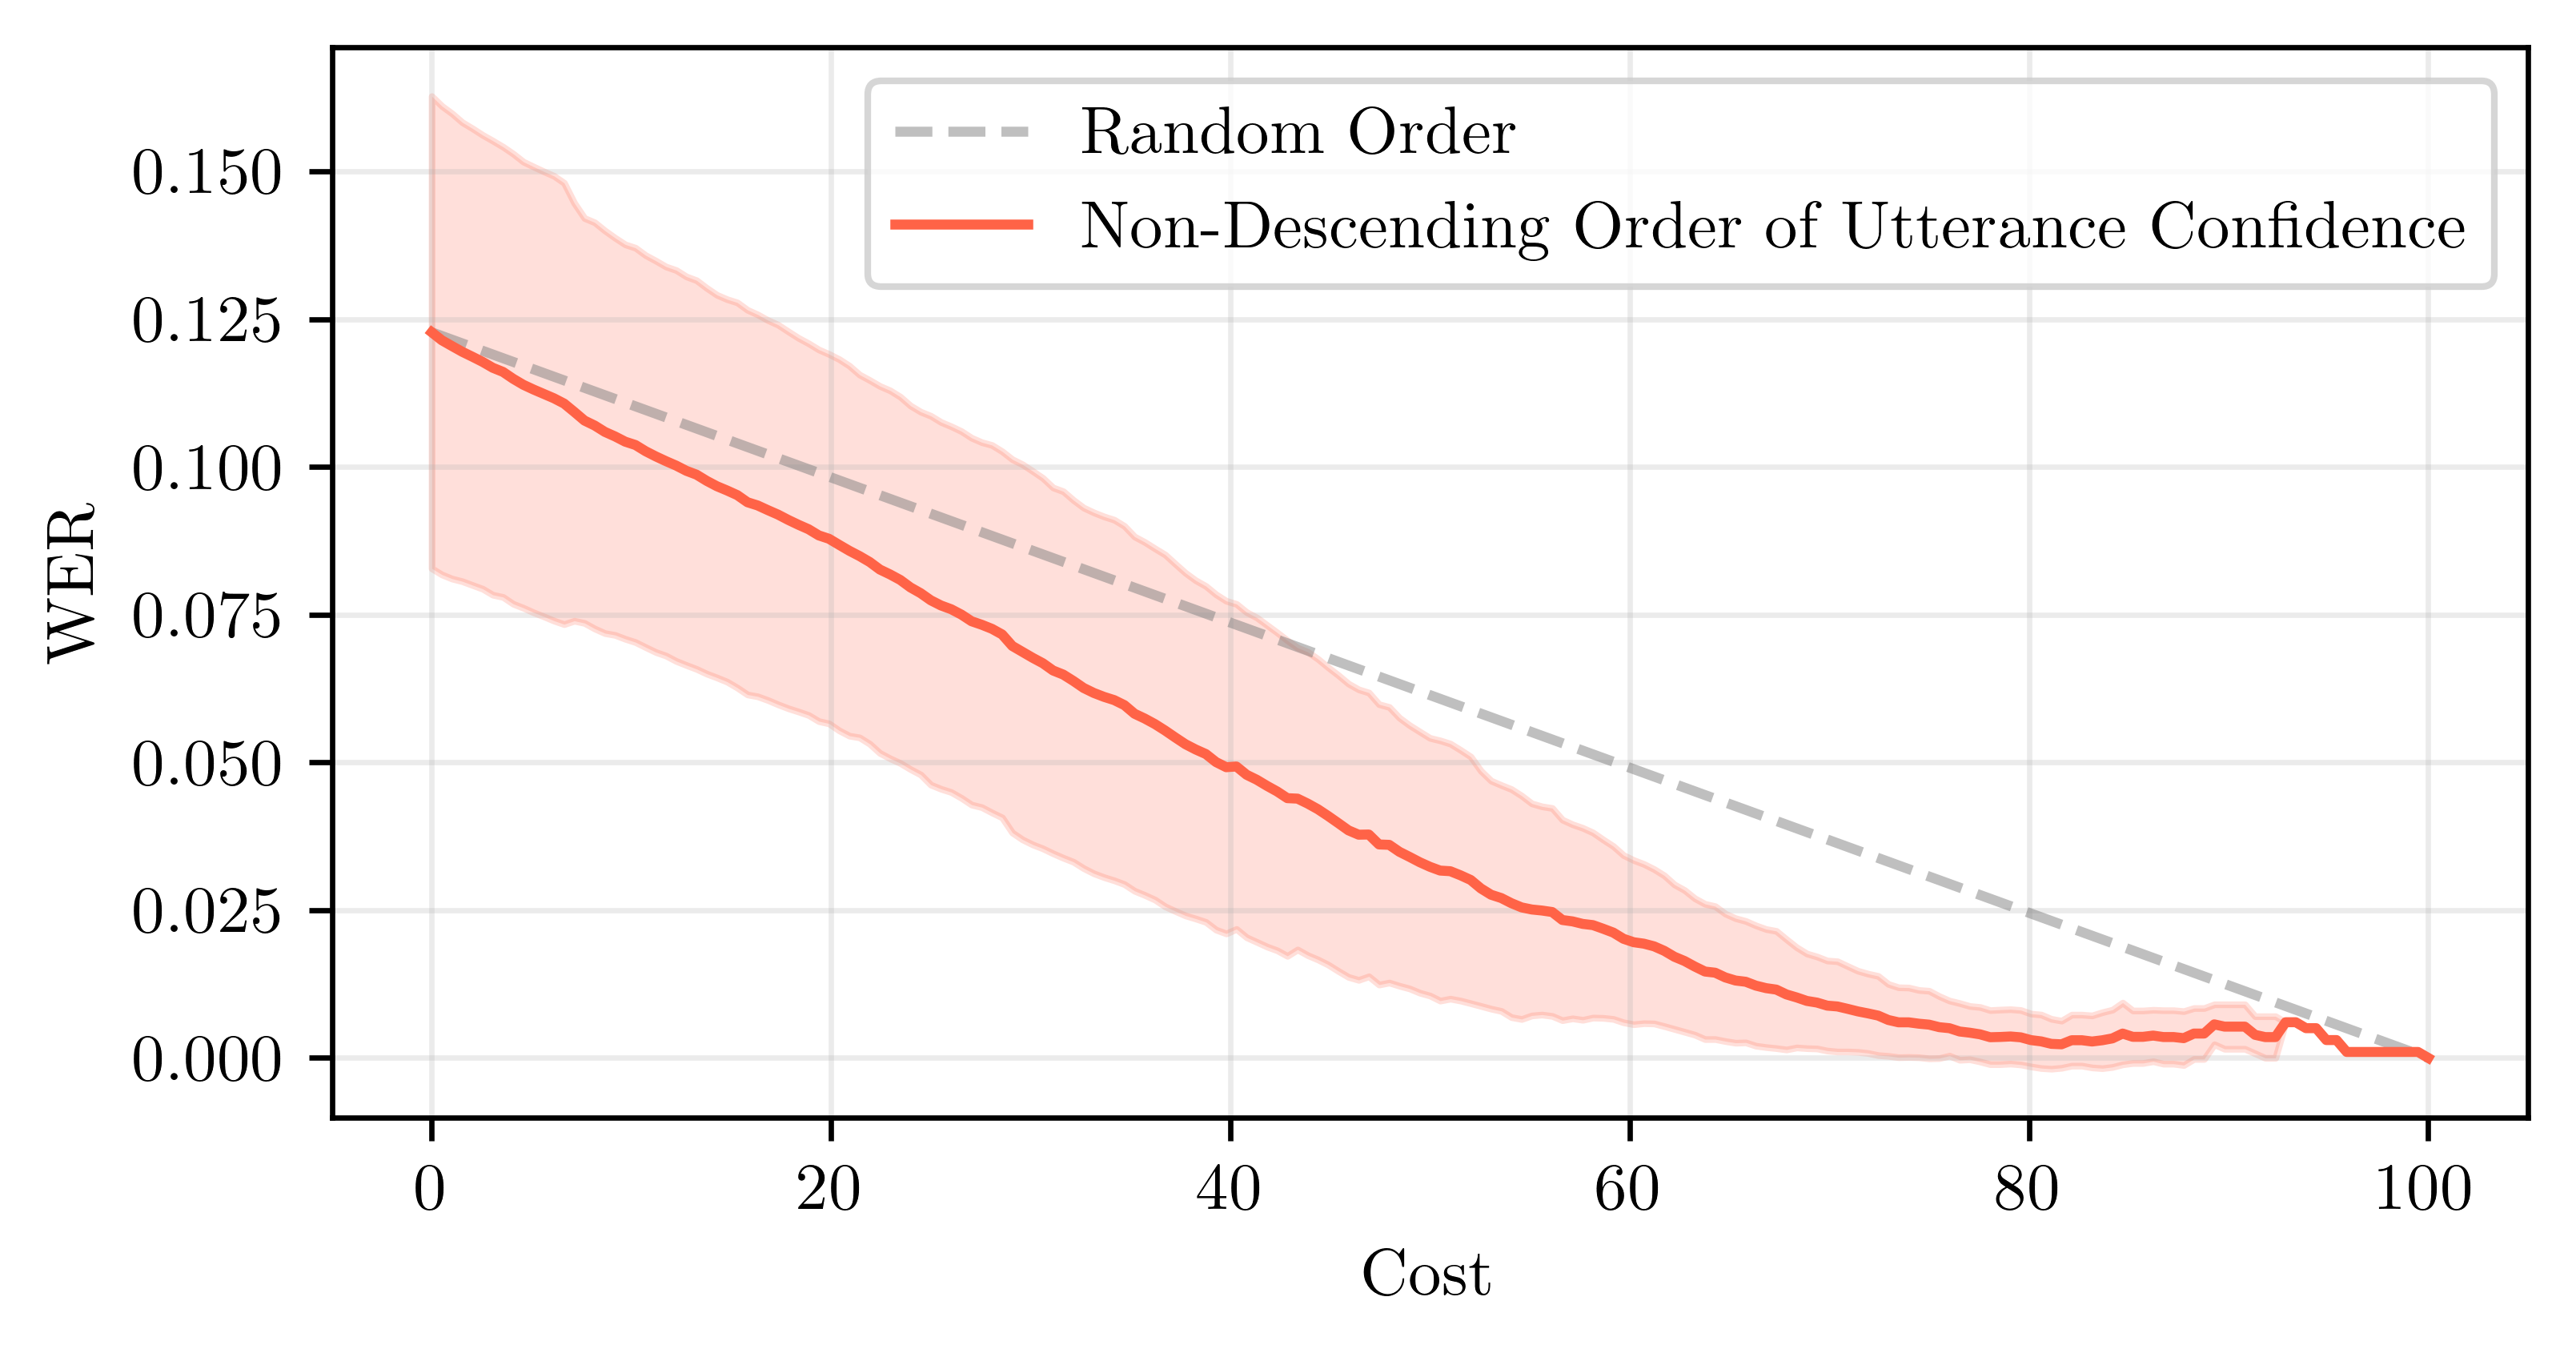
\includegraphics[width=\textwidth]{figures/average-uttconf.png}
 \centering
\end{figure}
\begin{figure}[p]
 \caption{Comparing per-conversation average performance of confidence and \texttt{avg\_logprob}}
 \label{fig:compare-avg-uttconf-vs-lprob}
 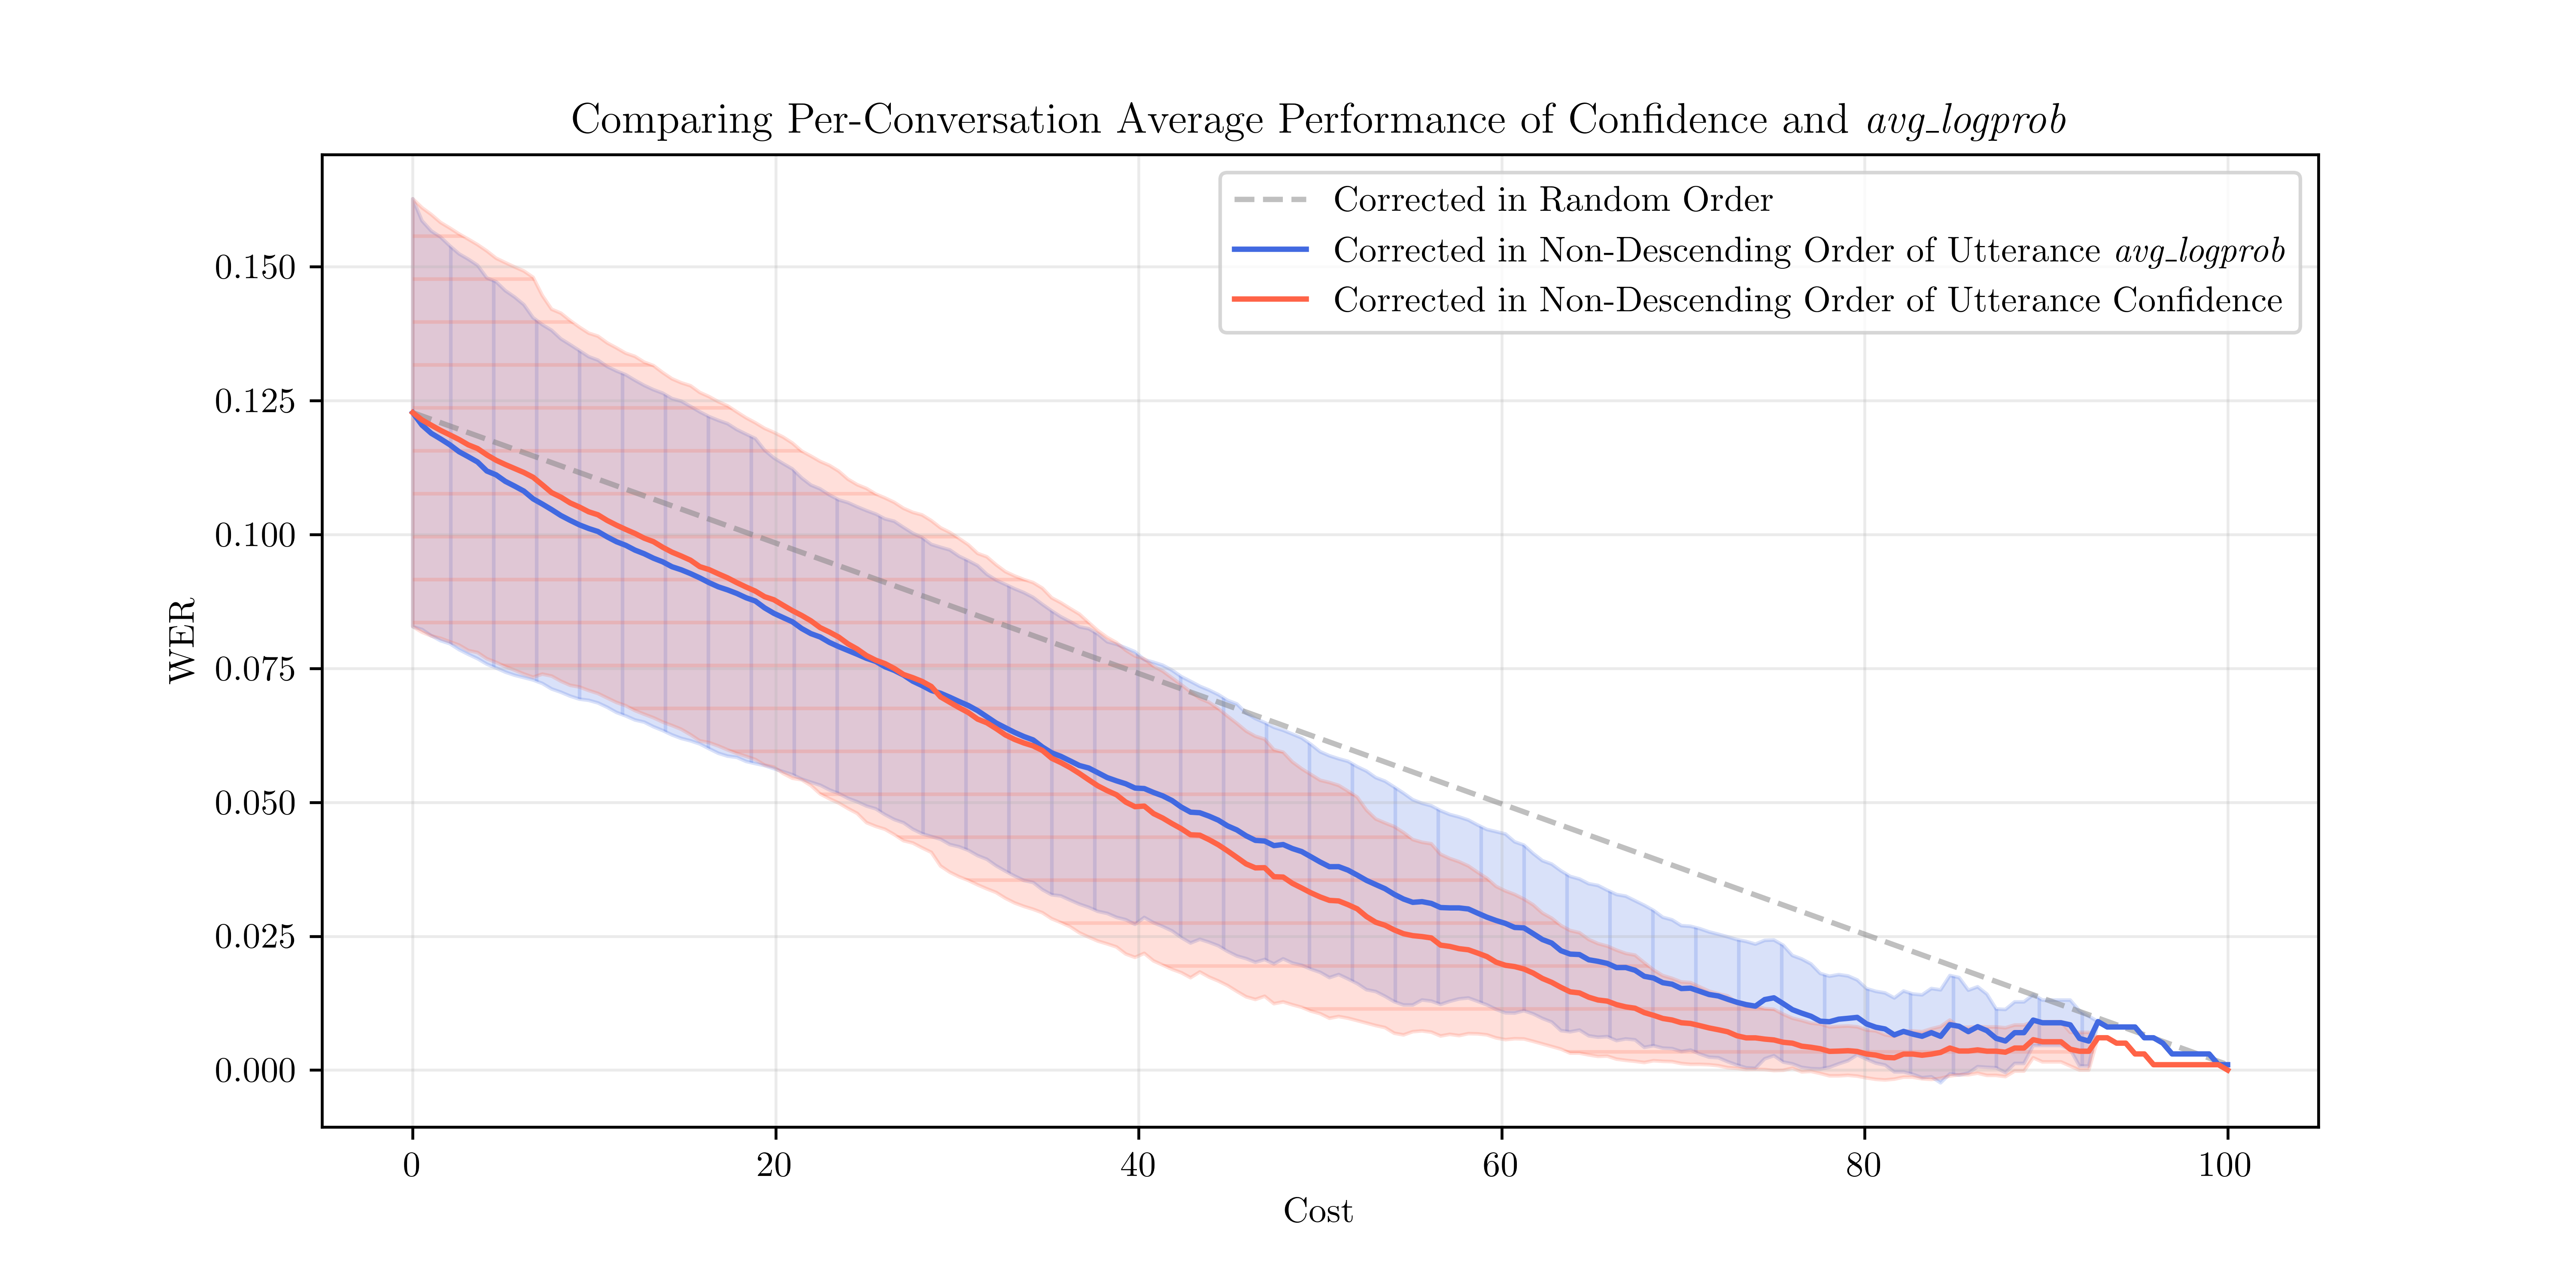
\includegraphics[width=\textwidth]{figures/compare-avg-uttconf-vs-lprob.png}
 \centering
\end{figure}
\begin{figure}[p]
 \caption{Comparing whole-corpus performance of confidence and \texttt{avg\_logprob}}
 \label{fig:corpus-avg-lprob-uttconf}
 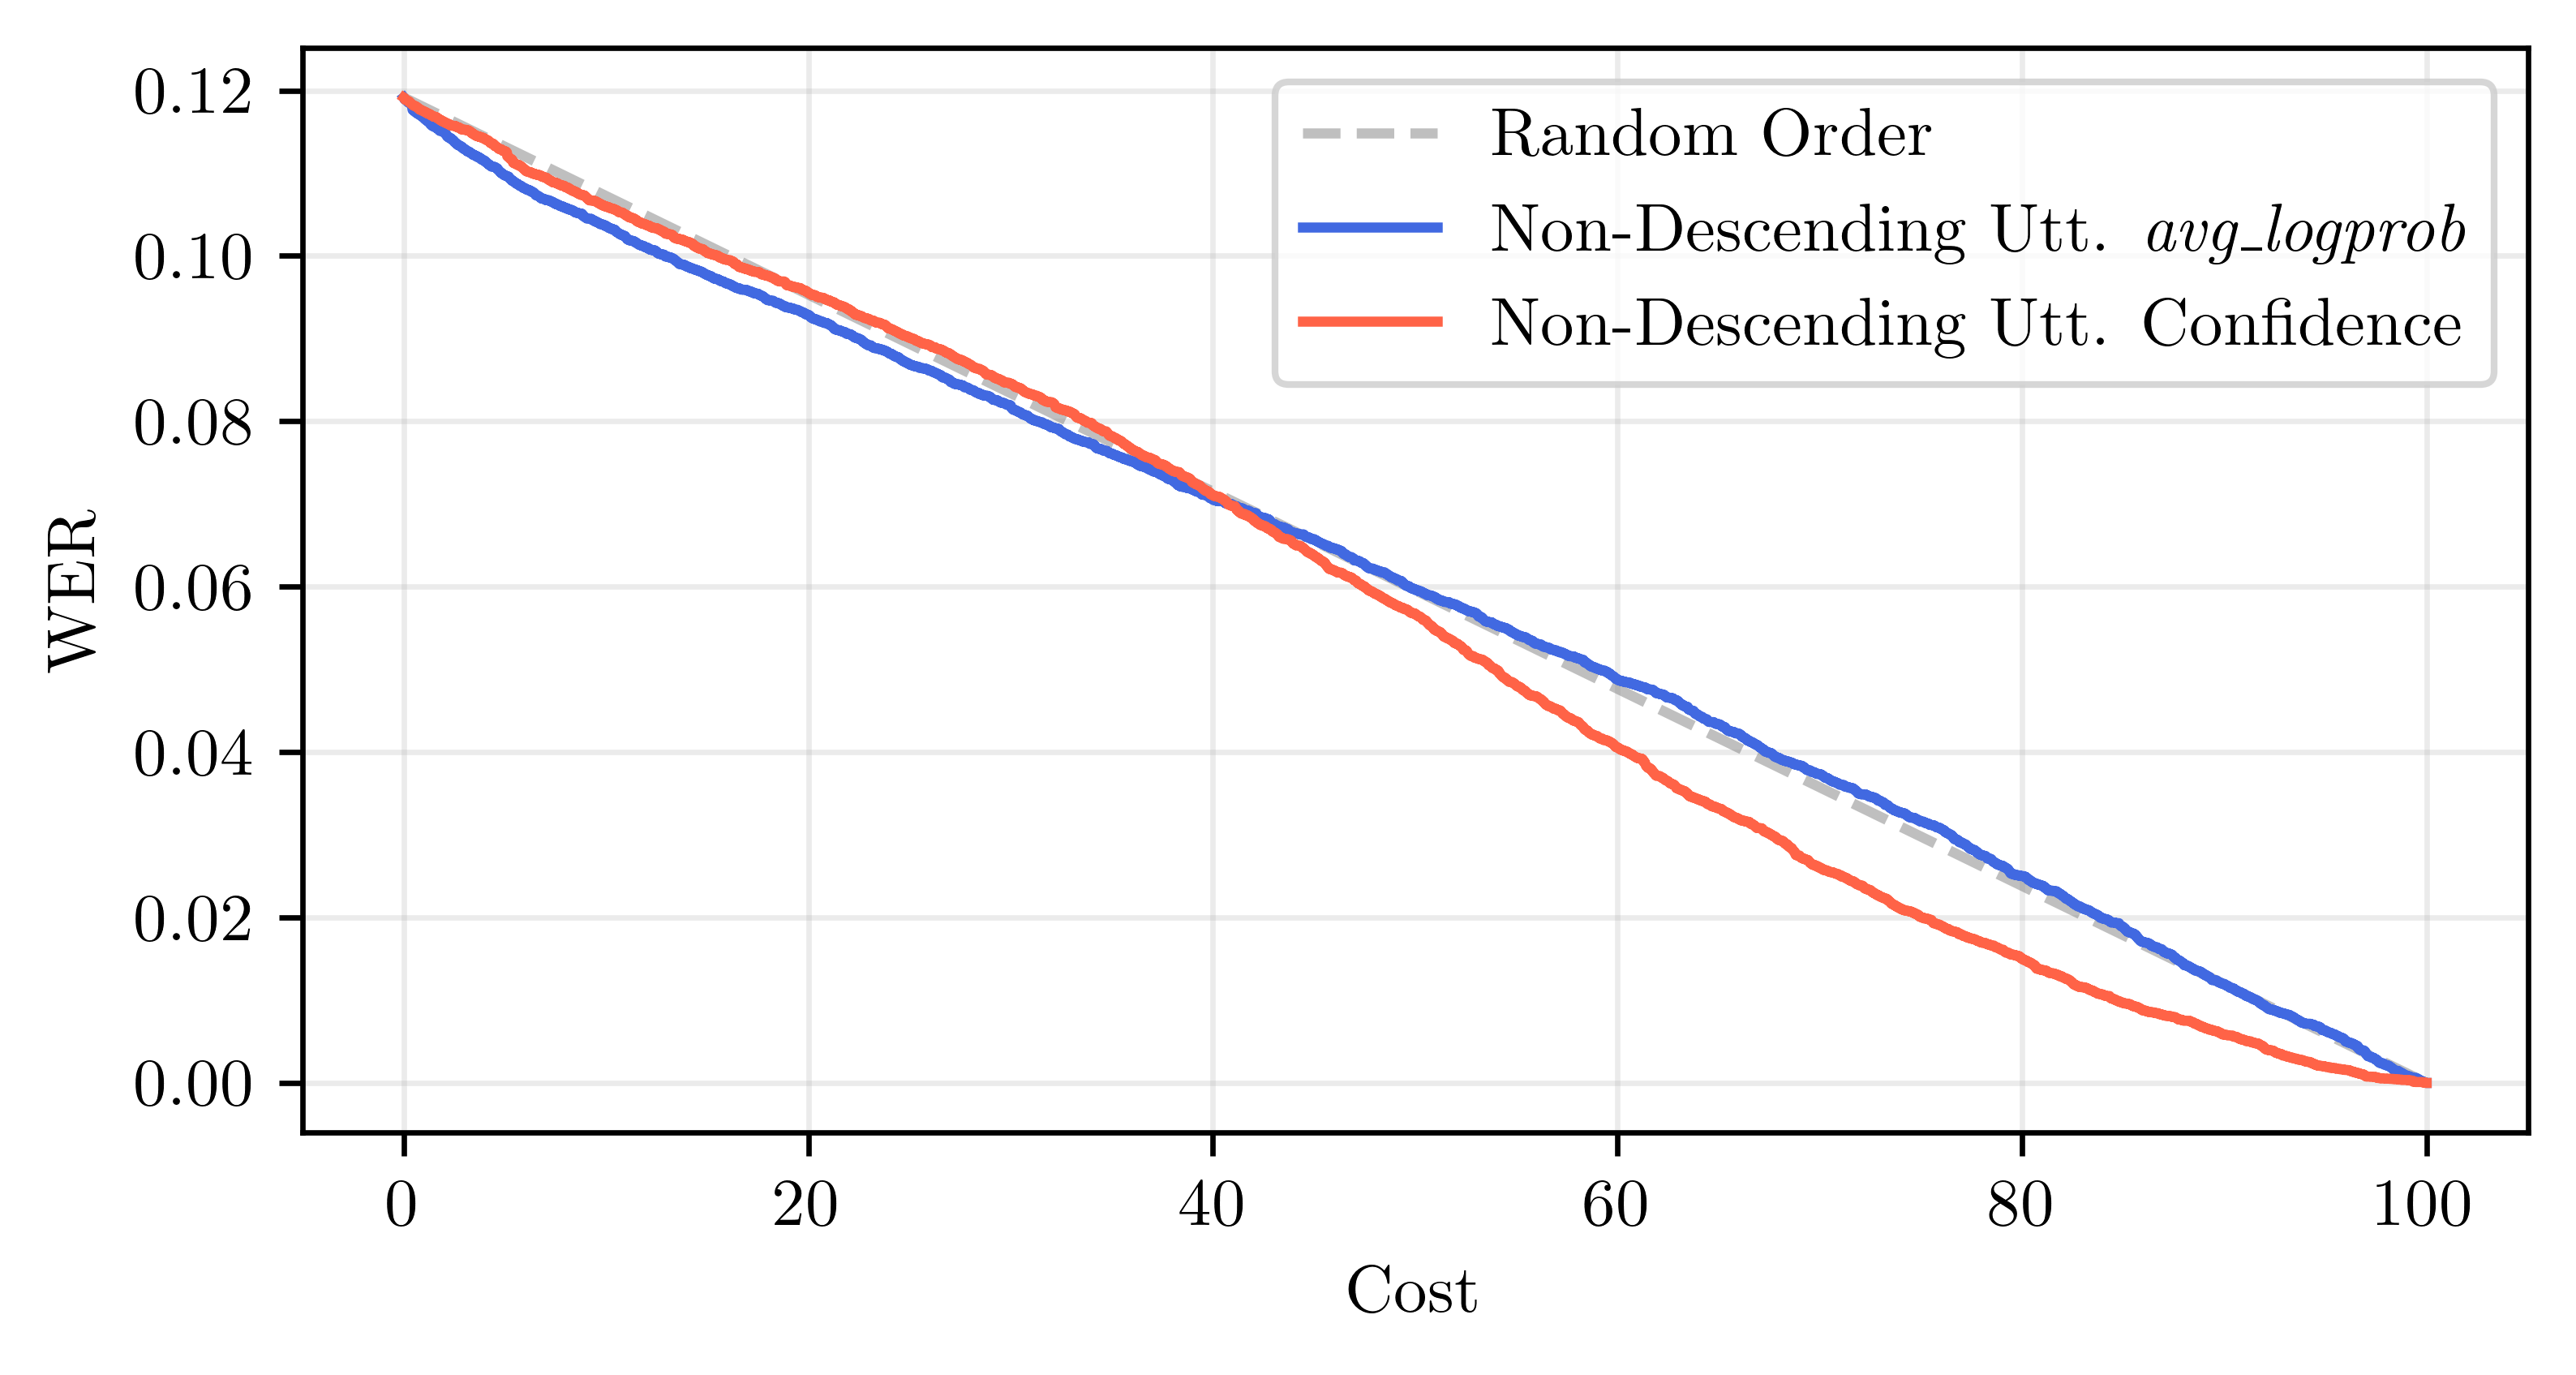
\includegraphics[width=\textwidth]{figures/corpus-avg-lprob-uttconf.png}
 \centering
\end{figure}

\clearpage
\subsection{Per-conversation average results using word-confidence}

\begin{figure}[h!]
 \caption{Ordered by non-descending utterance-minimum word-confidence}
 \label{fig:word-conf-comparison-plot1}
 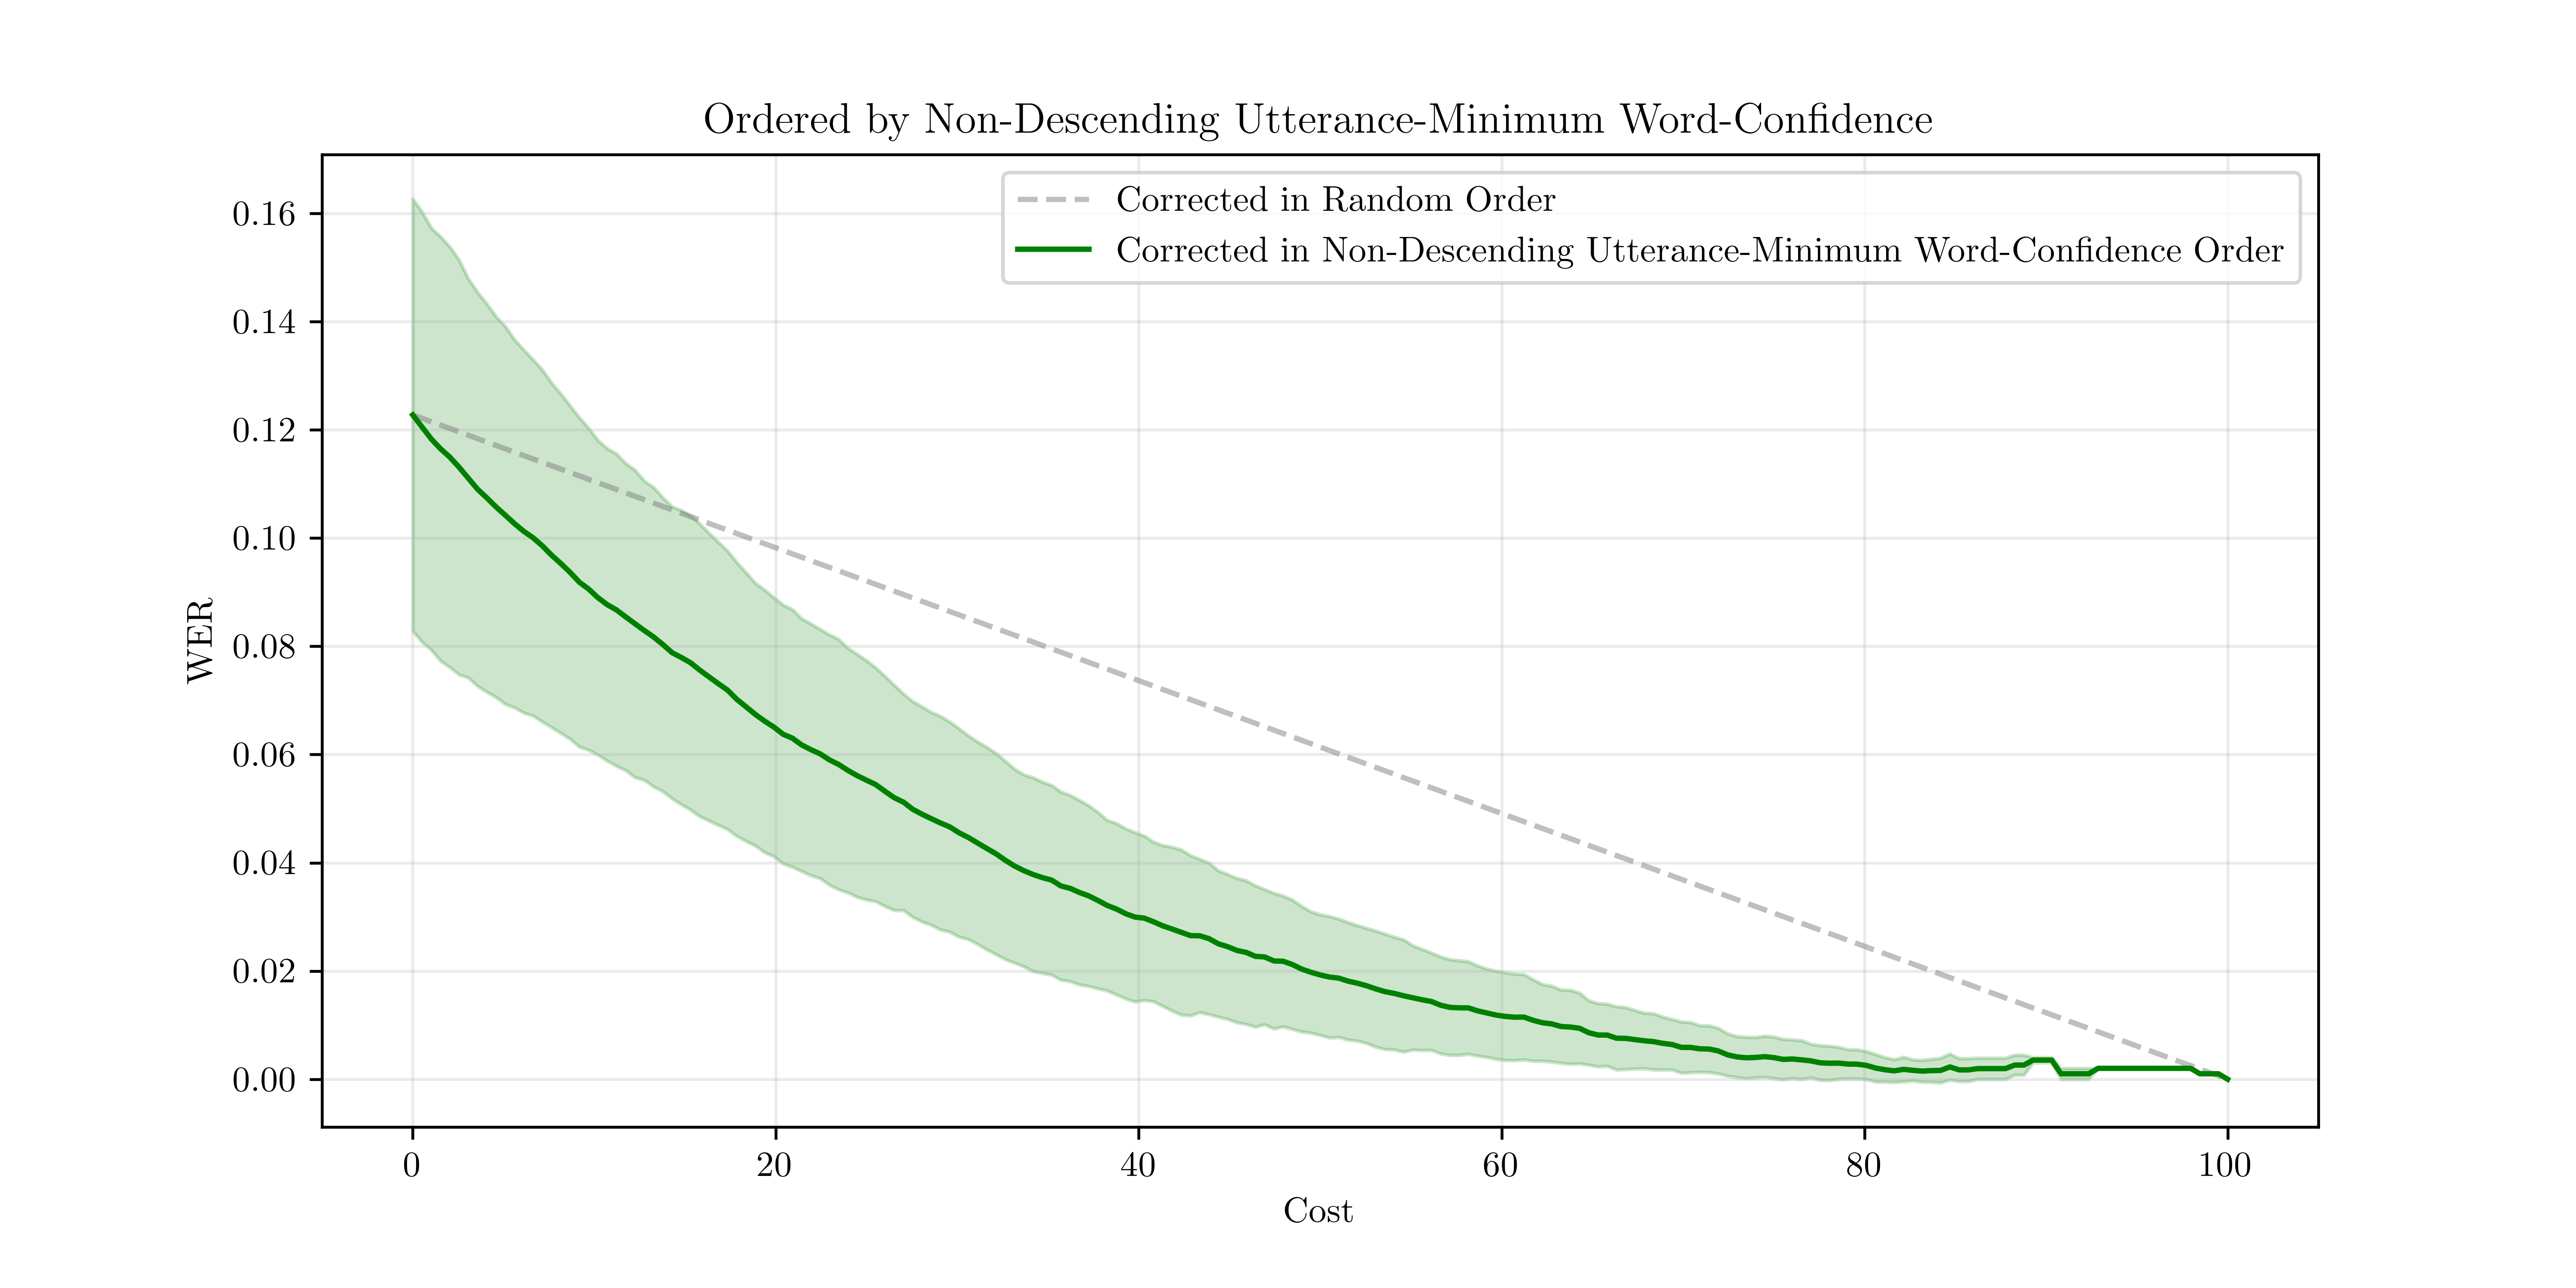
\includegraphics[width=\textwidth]{figures/word-conf-comparison-plot1.png}
 \centering
\end{figure}
\begin{figure}[h!]
 \caption{Ordered by non-ascending utterance-minimum word-confidence}
 \label{fig:word-conf-comparison-plot2}
 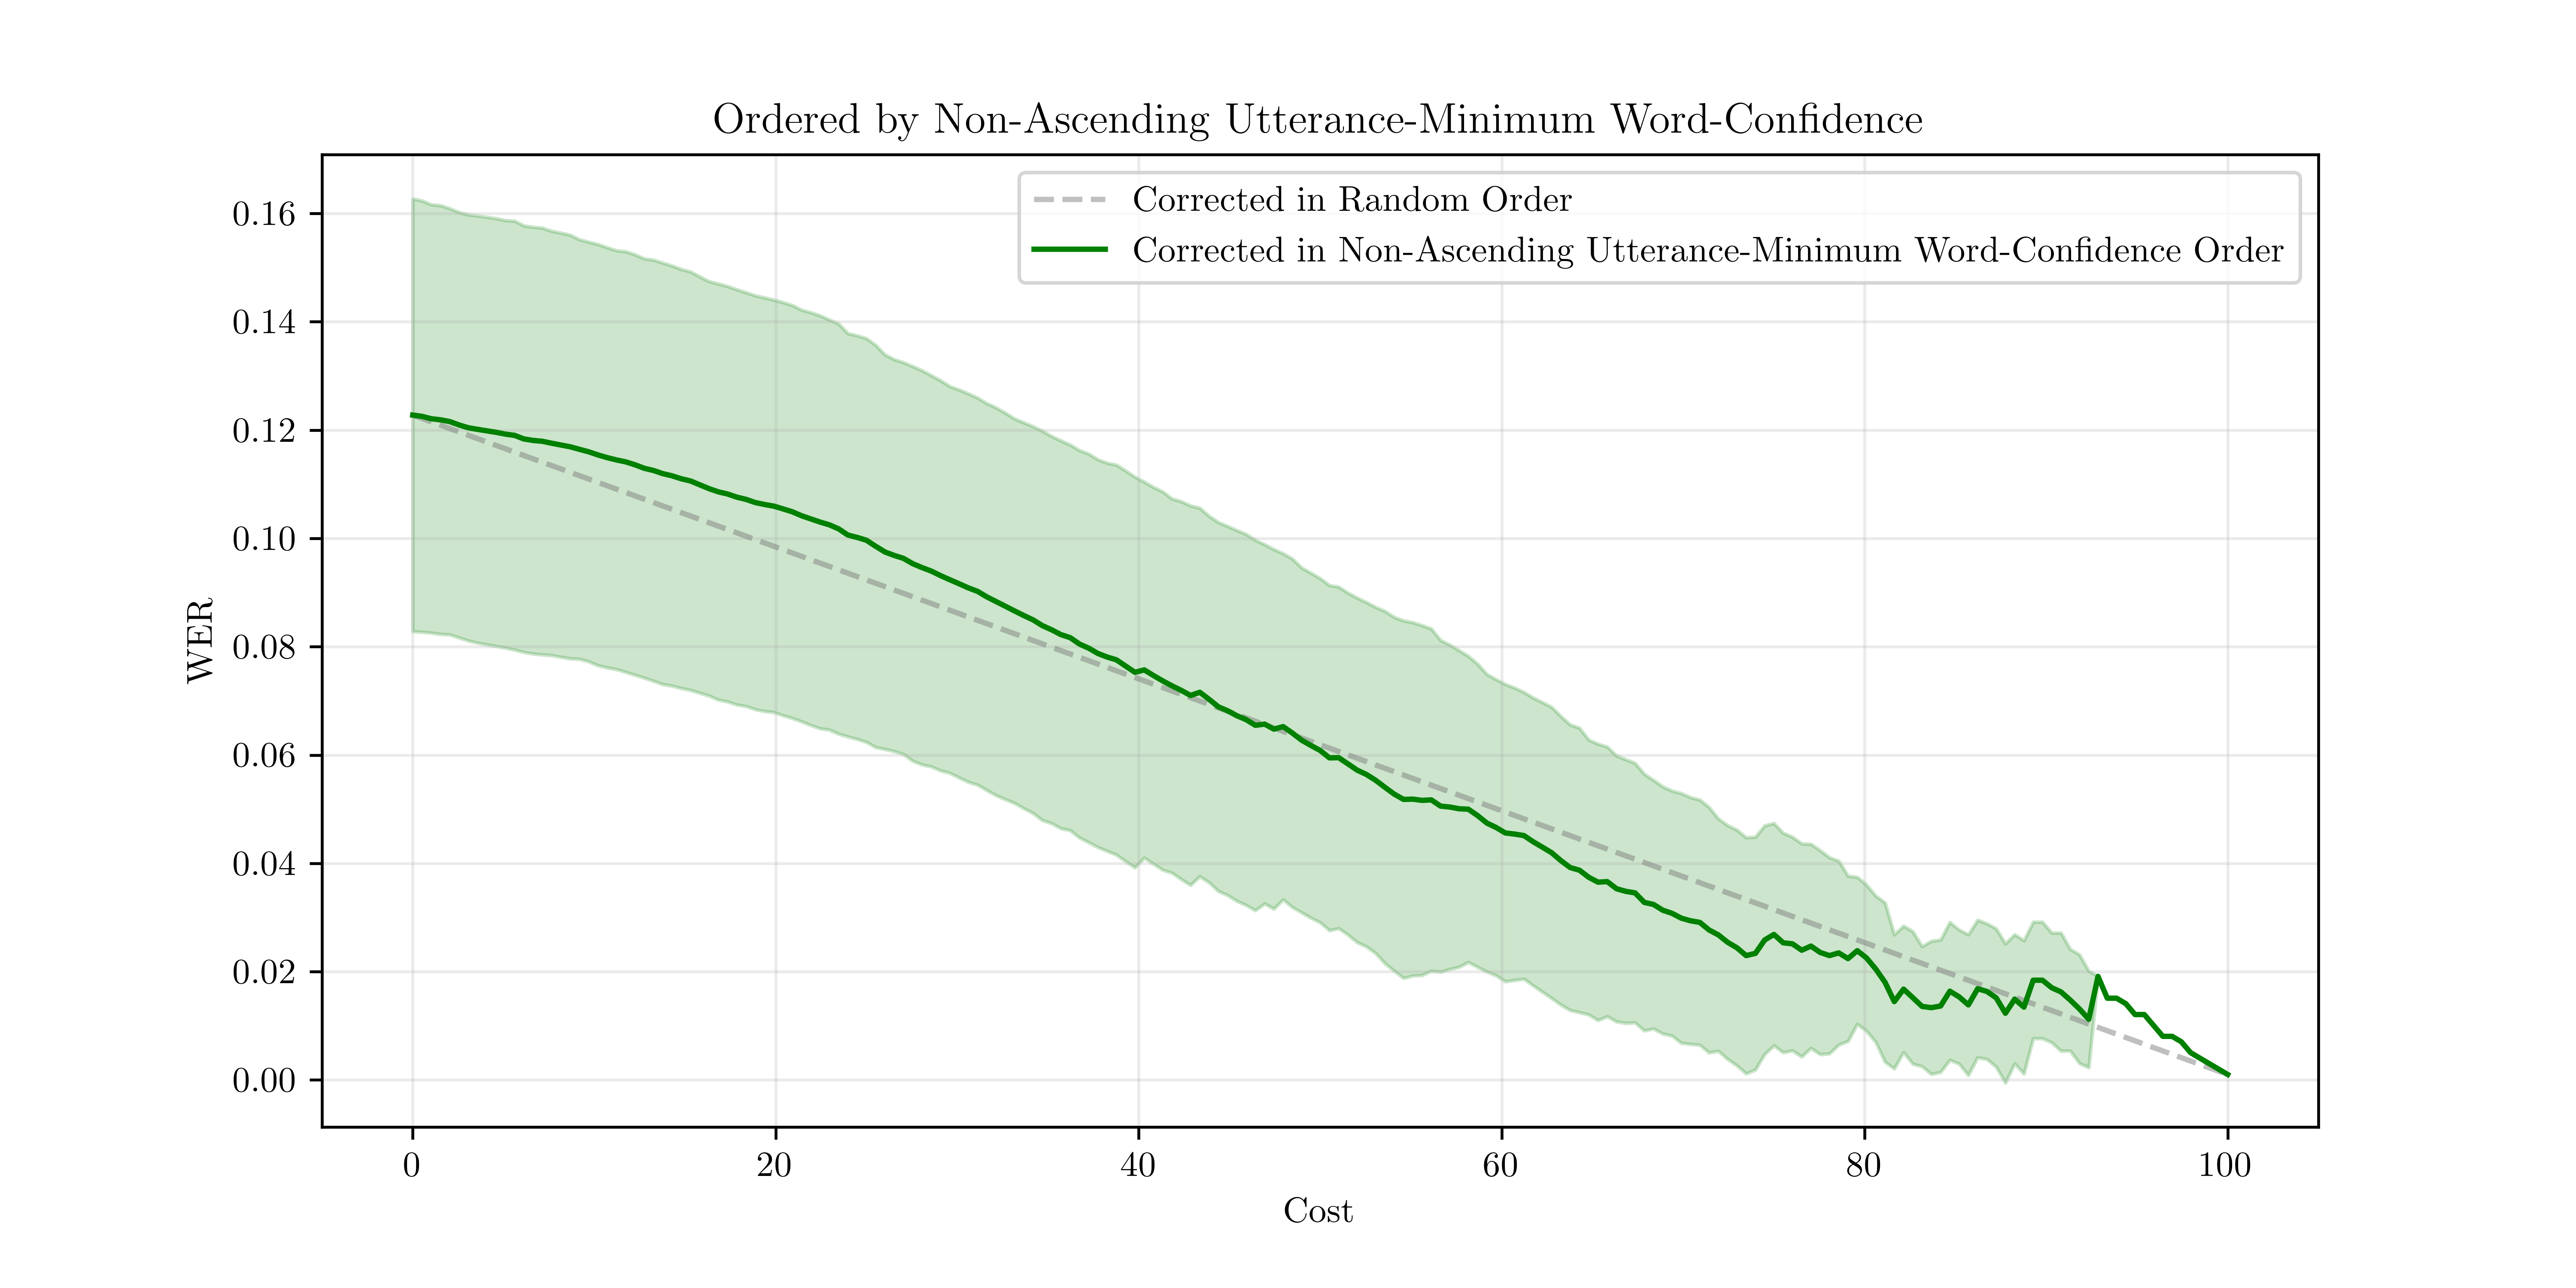
\includegraphics[width=\textwidth]{figures/word-conf-comparison-plot2.png}
 \centering
\end{figure}
\begin{figure}[p]
 \caption{Ordered by non-descending utterance-maximum word-confidence}
 \label{fig:word-conf-comparison-plot3}
 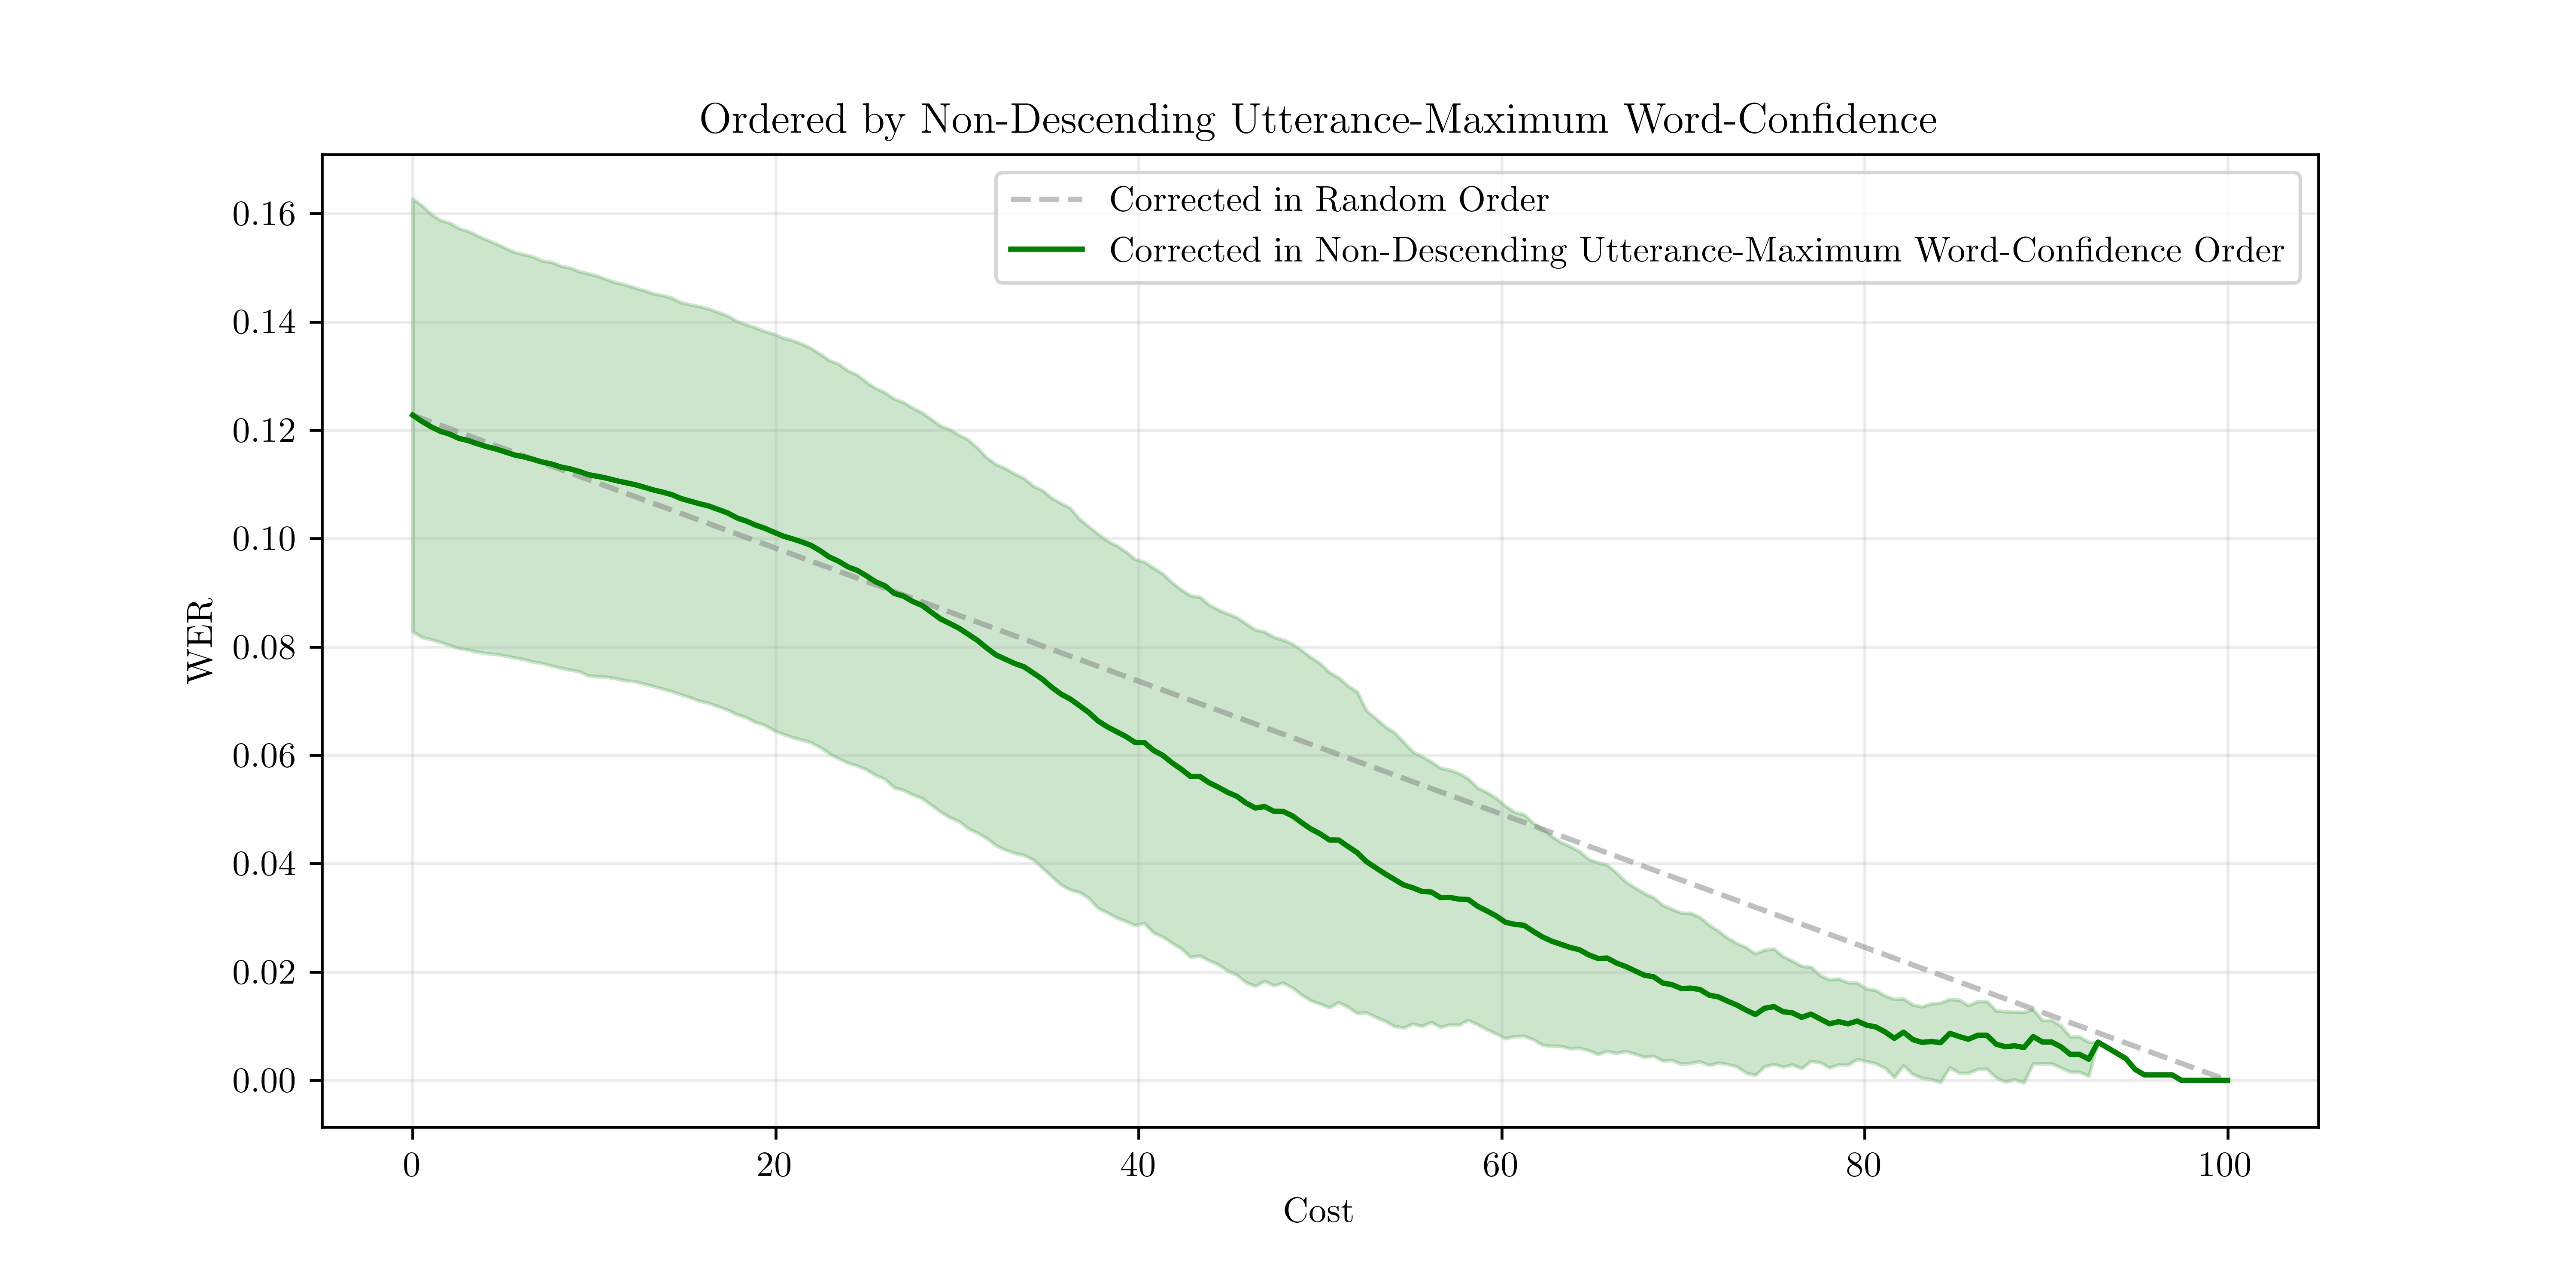
\includegraphics[width=\textwidth]{figures/word-conf-comparison-plot3.png}
 \centering
\end{figure}
\begin{figure}[p]
 \caption{Ordered by non-ascending utterance-maximum word-confidence}
 \label{fig:word-conf-comparison-plot4}
 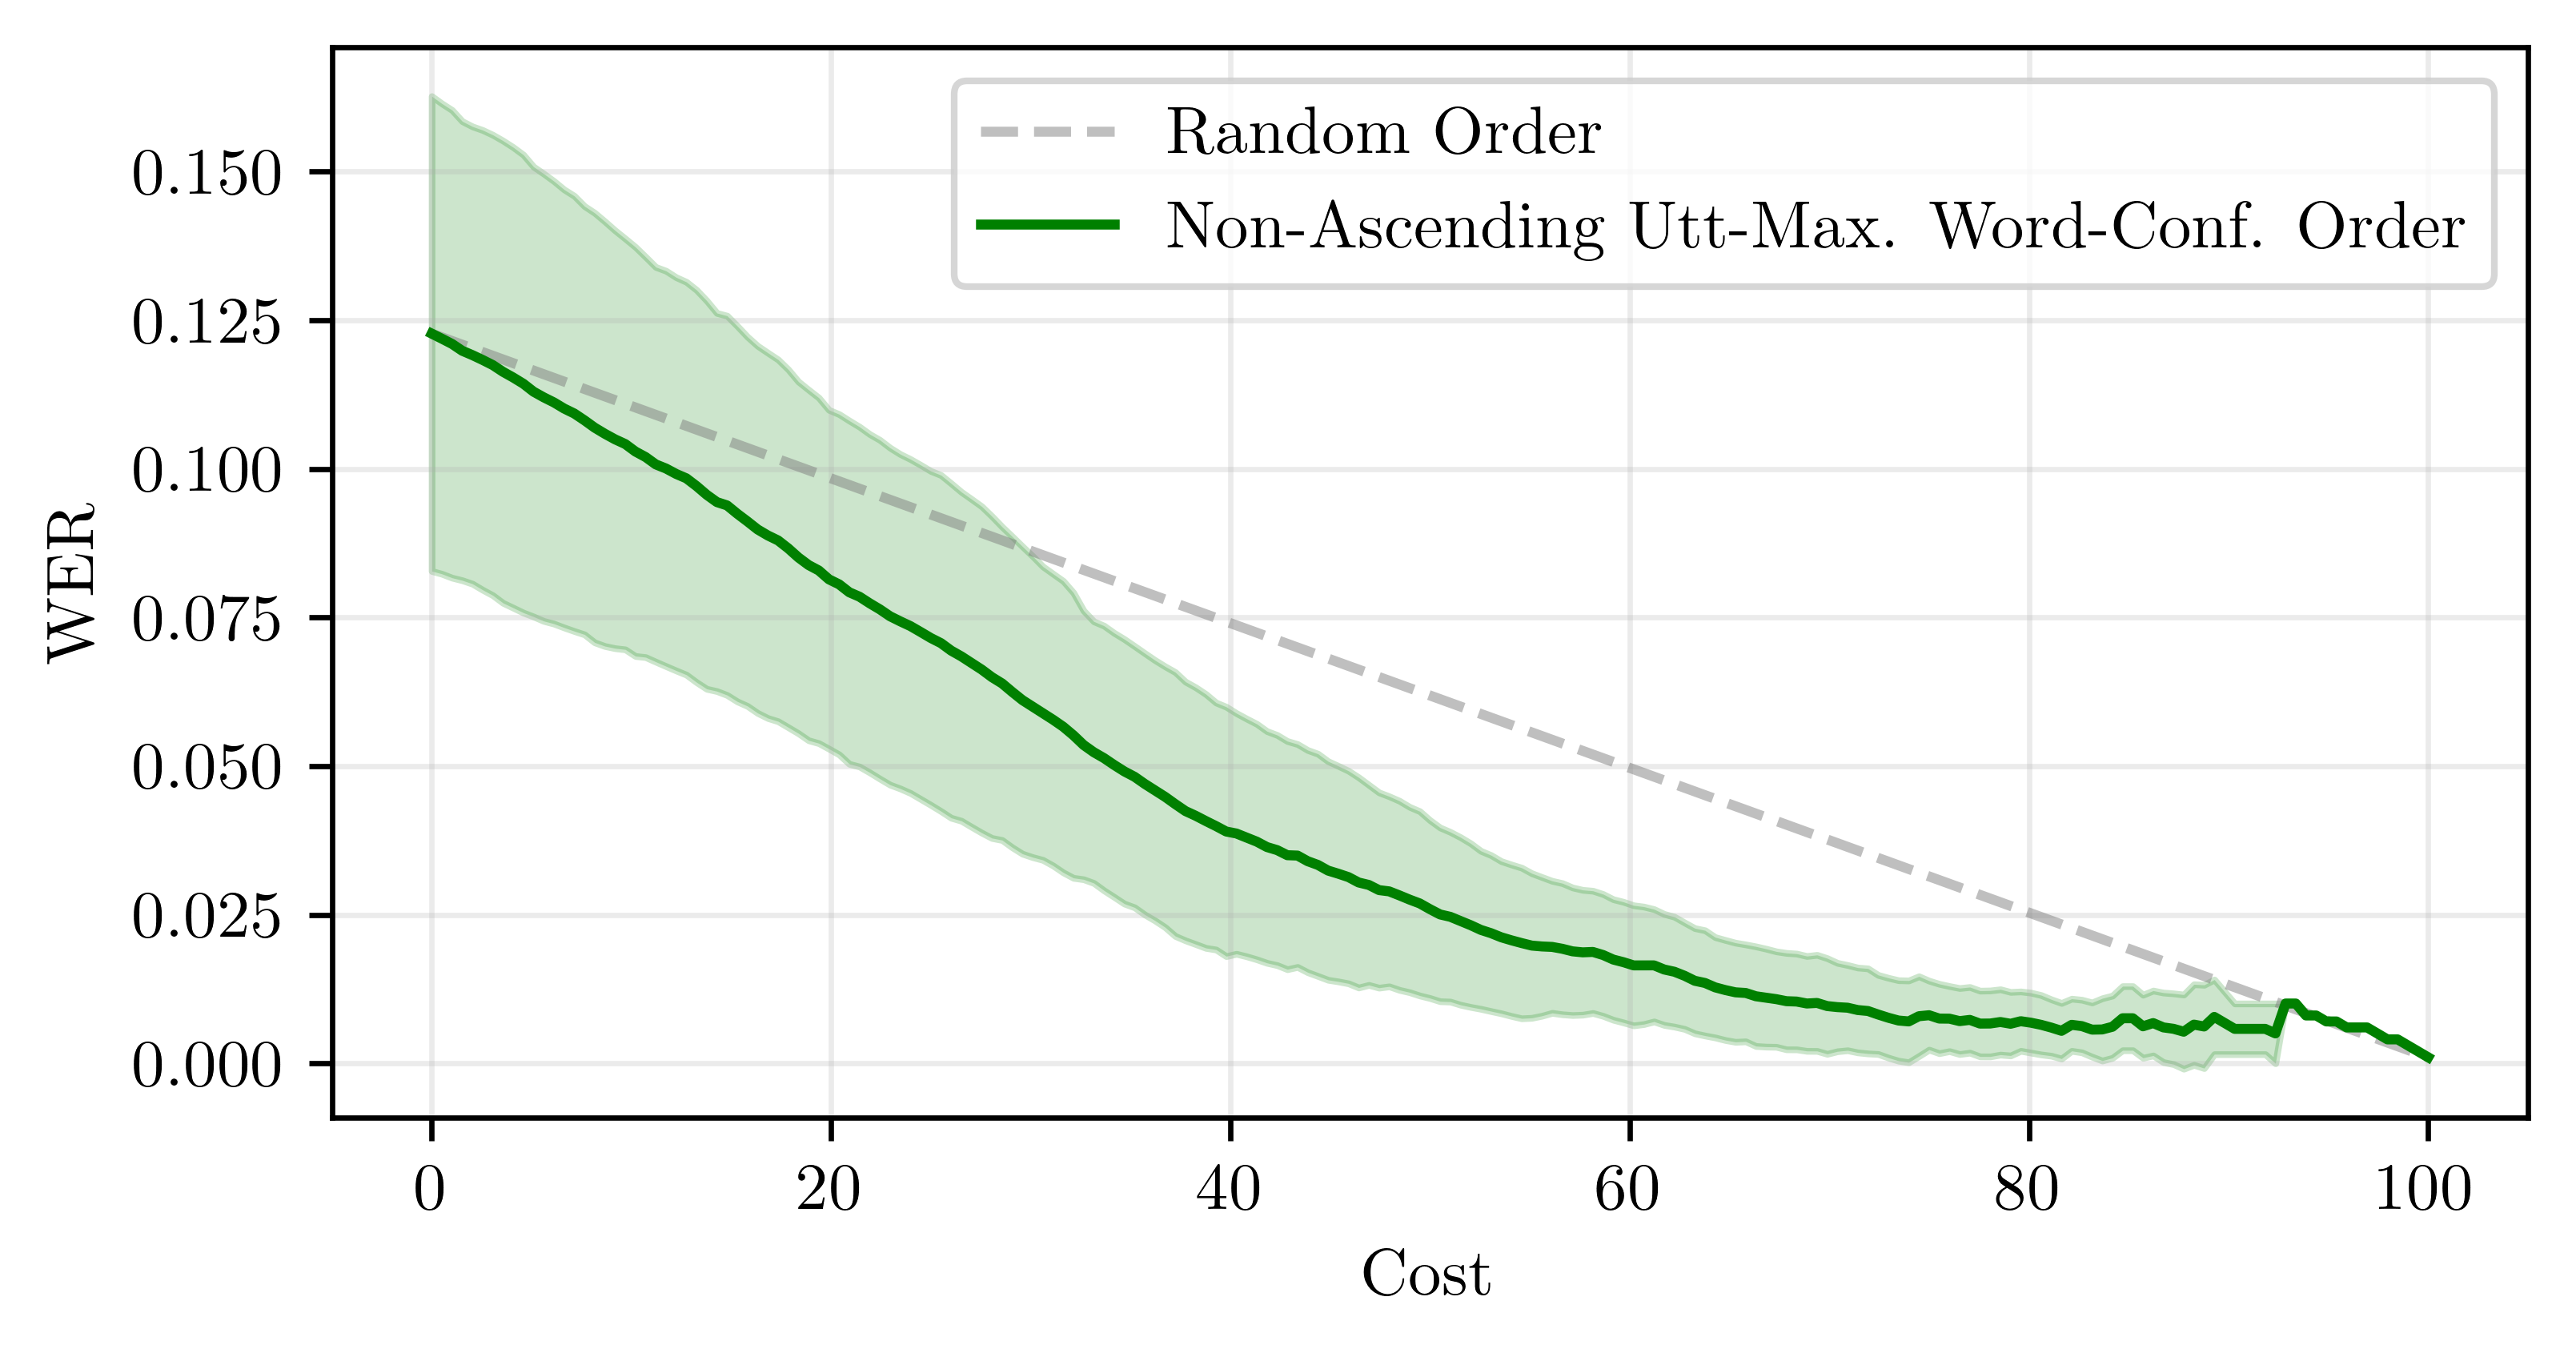
\includegraphics[width=\textwidth]{figures/word-conf-comparison-plot4.png}
 \centering
\end{figure}

\clearpage
\subsection{Comparisons between all measures}

\begin{figure}[h!]
 \caption{}
 \label{fig:}
 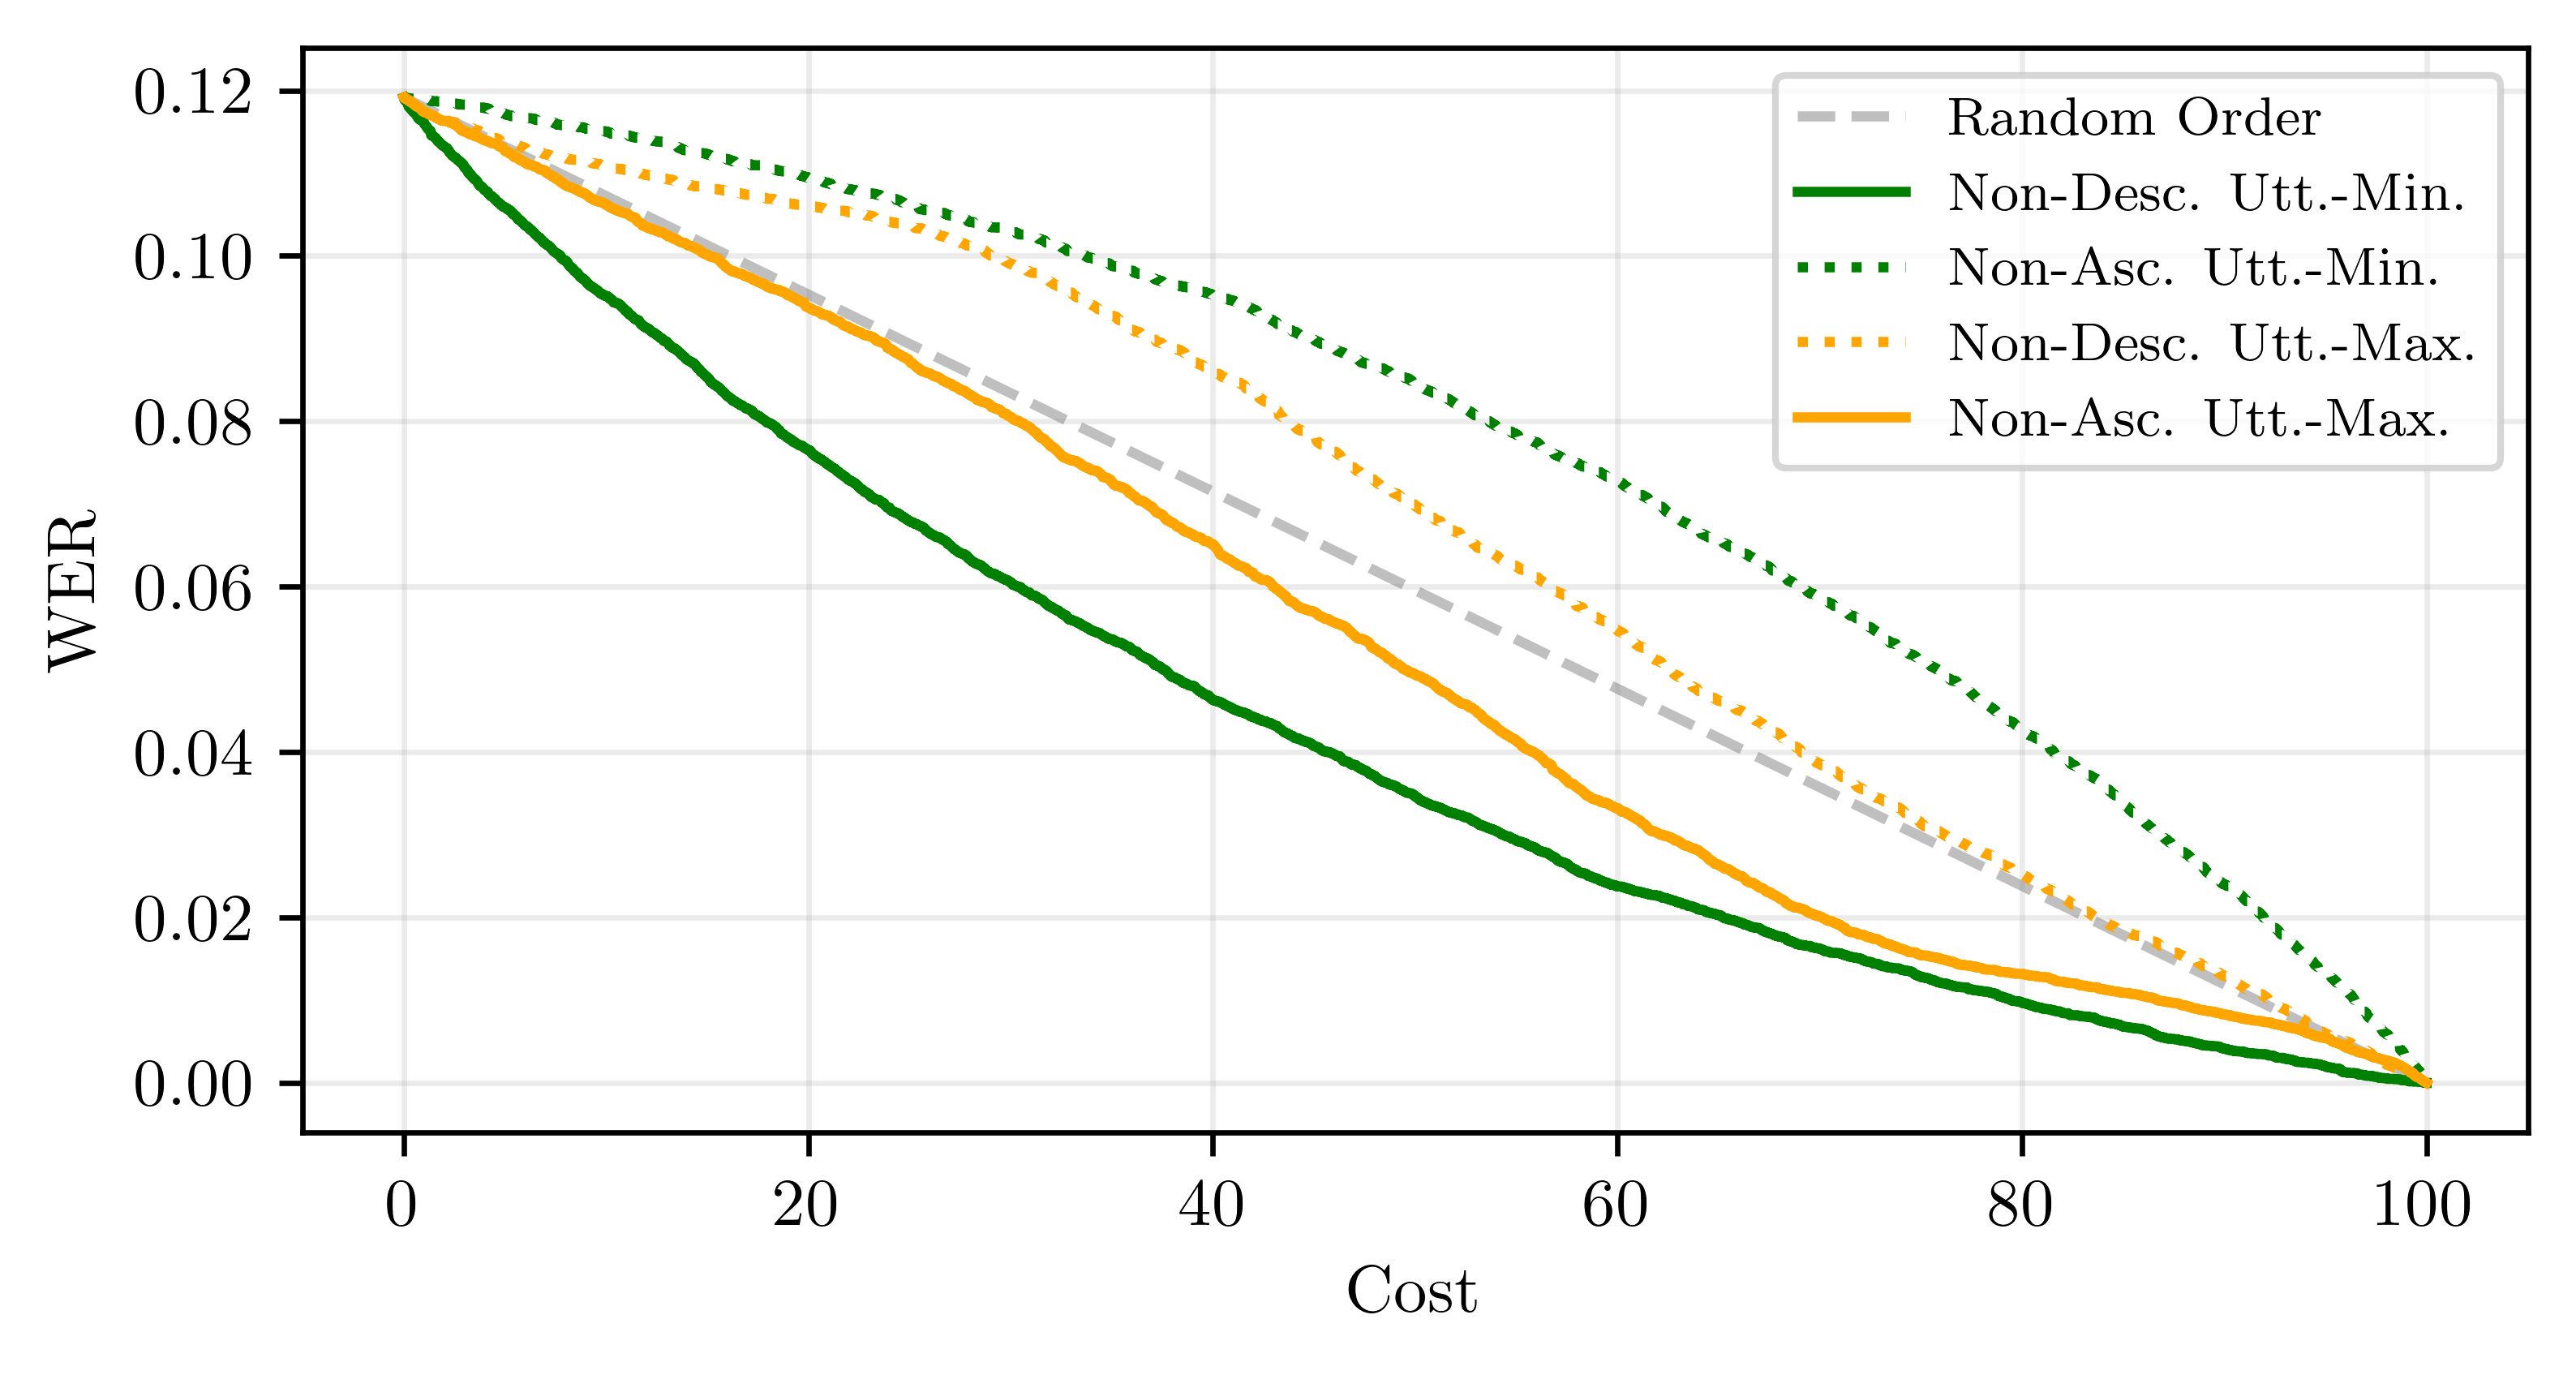
\includegraphics[width=\textwidth]{figures/corpus-all-word-conf-measures.png}
 \centering
\end{figure}
\begin{figure}[h!]
 \caption{}
 \label{fig:}
 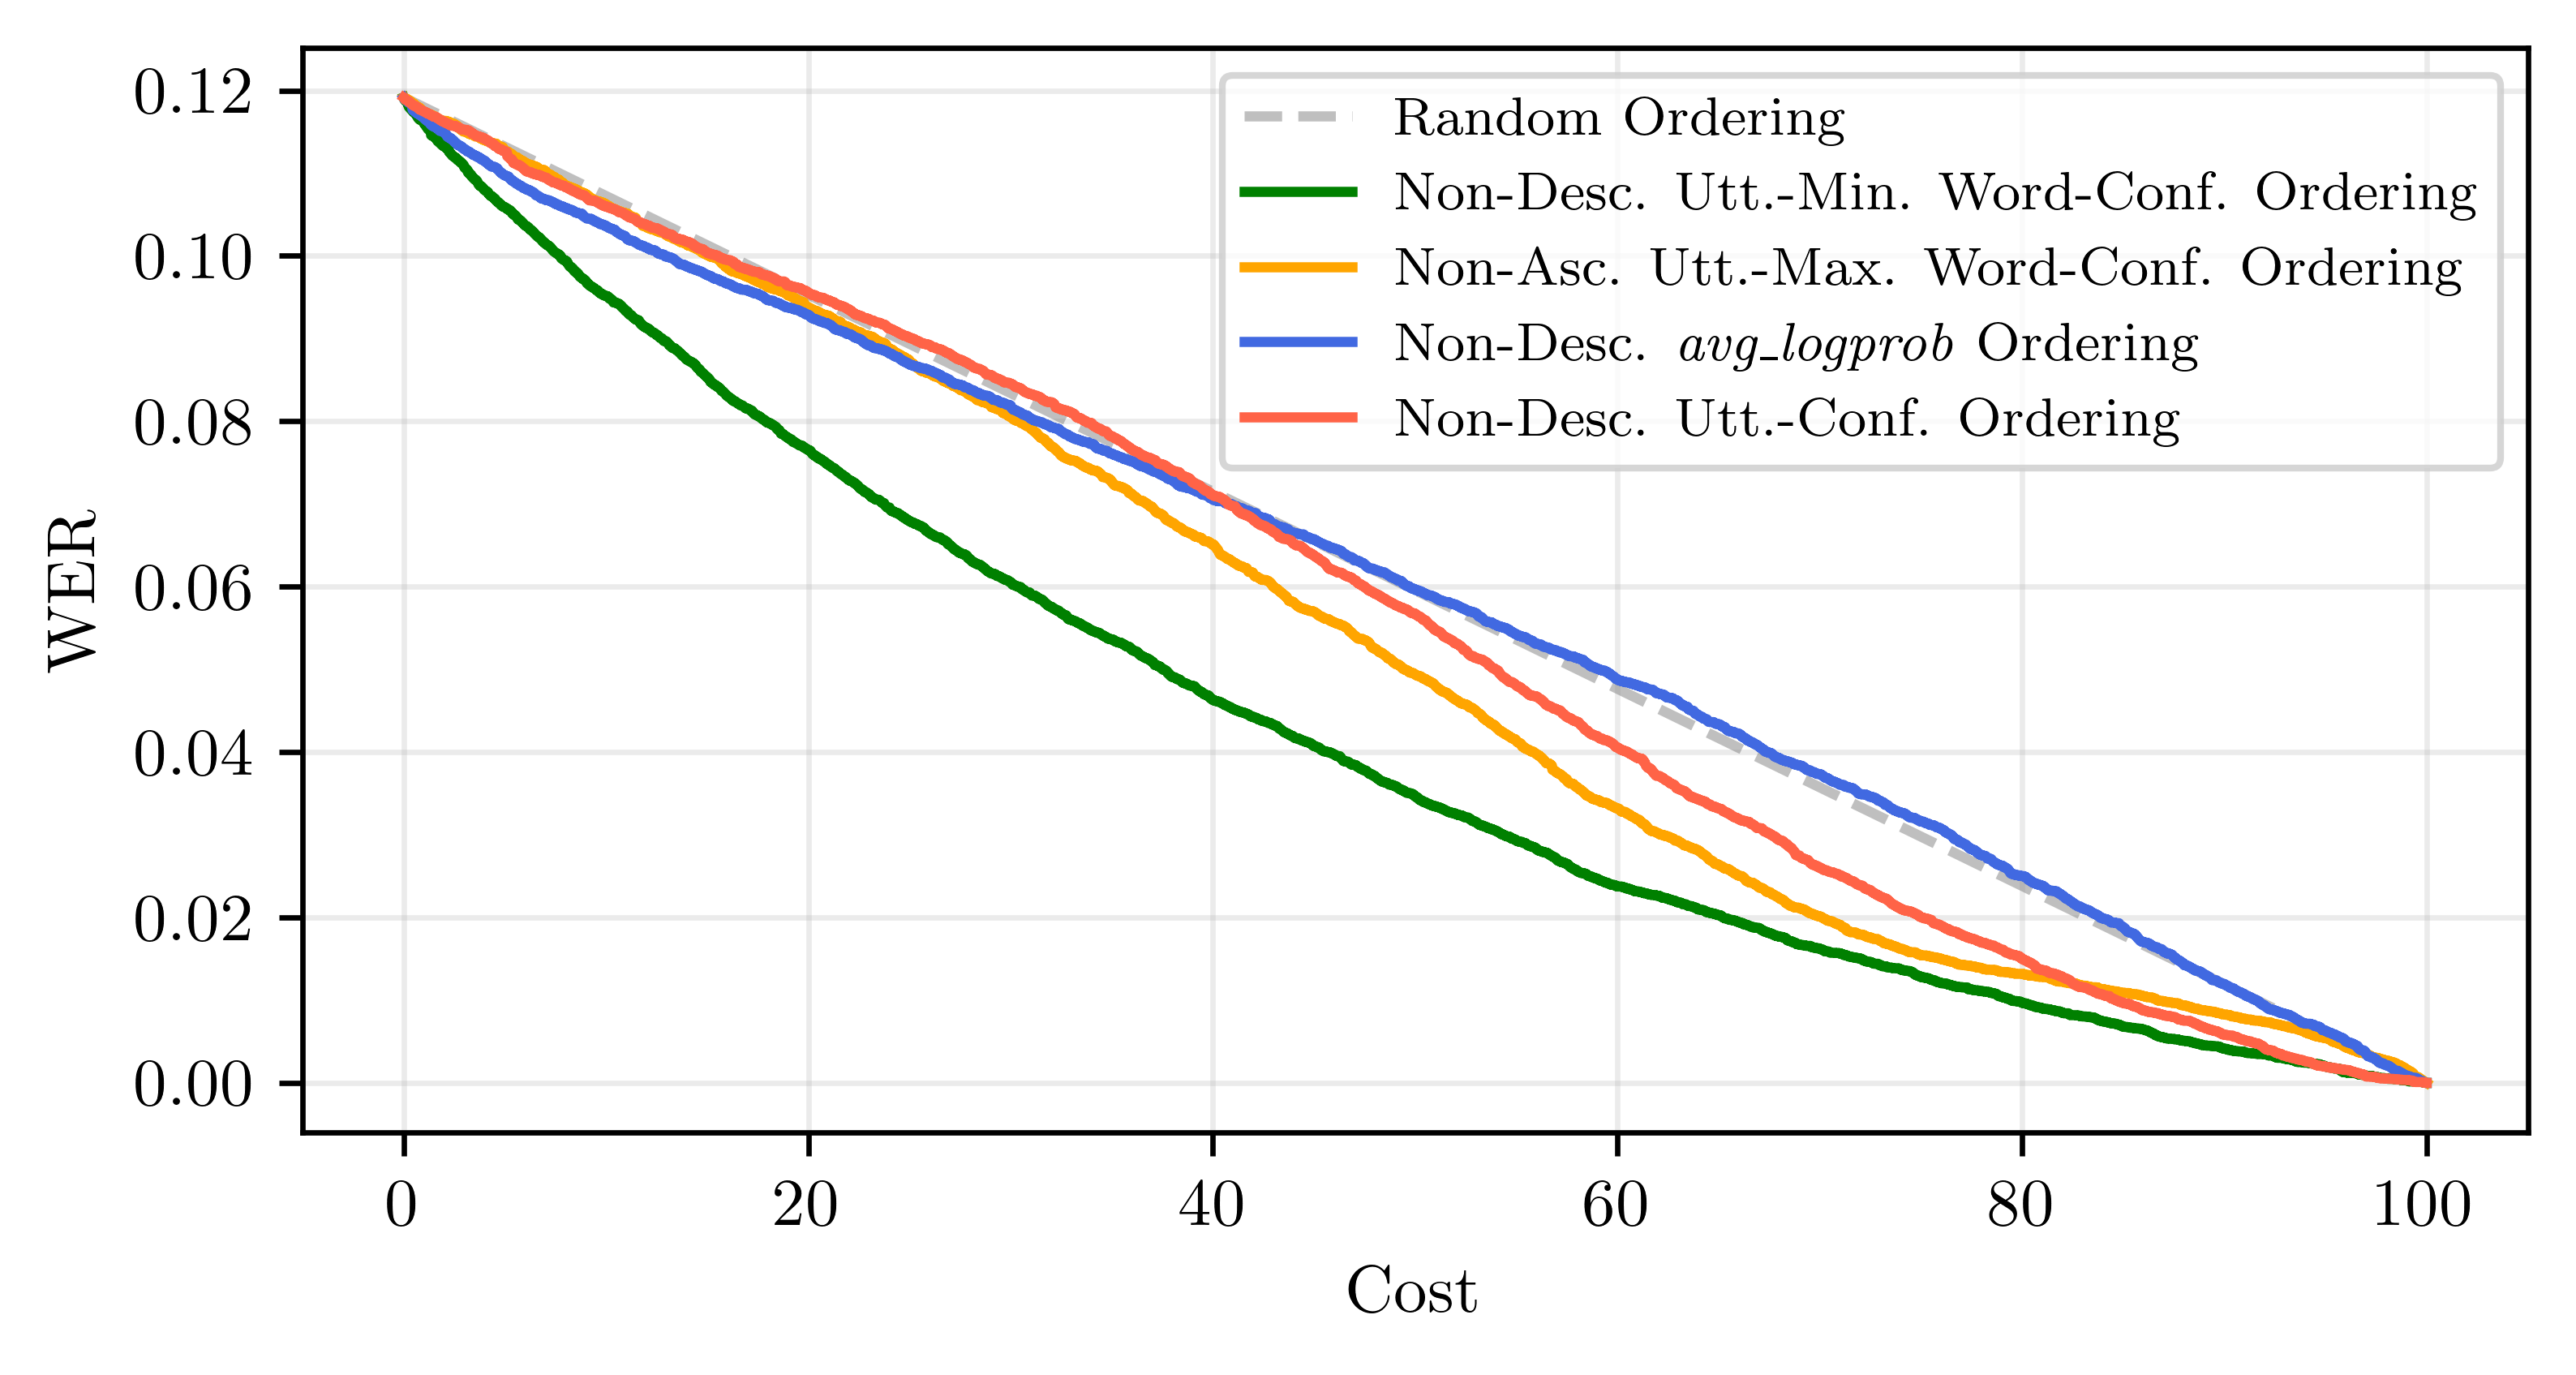
\includegraphics[width=\textwidth]{figures/corpus-allmeasures.png}
 \centering
\end{figure}

\clearpage
\section{Discussion of Results}
In this section ...
